\chapter{Eclipse y Scene Builder}
\section{Contenidos en Parte 1}
\begin{itemize}
	\item Familiarizándose con JavaFX.
	\item Crear y empezar un proyecto JavaFX.
	\item Uso de Scene builder para diseñar la interfaz de usuario
	\item Estructura básica de una aplicación mediante el patrón Modelo Vista Controlador (MVC).
\end{itemize}

\section{Prerrequisitos}
\begin{itemize}
	\item Última versión de \textcolor{azul}{\href{https://www.oracle.com/java/technologies/javase-downloads.html}{Java JDK 8 o superior}}.
	\item Eclipse 4.3 o superior con el plugin e(fx)clipse. La forma más sencilla de obtenerlo es descargarse la distribución preconfigurada desde \textcolor{azul}{\href{https://efxclipse.bestsolution.at/install.html\#all-in-one}{e(fx)clipse website}}. Como alternativa puedes usar un \textcolor{azul}{\href{https://www.eclipse.org/efxclipse/install.html}{sitio de actualización}} para tu instalación de Eclipse.
	\item \textcolor{azul}{\href{https://www.oracle.com/technetwork/java/javase/downloads/javafxscenebuilder-info-2157684.html}{Scene Builder 2.0}} o superior
\end{itemize}

\section{Configuración de Eclipse}
Hay que indicarle a Eclipse que use JDK 8 y también dónde se encuentra el ejecutable del Scene Builder:
\begin{enumerate}
	\item Abre las Preferencias de Eclipse (menú\textit{ Window | Preferences} y navega hasta \textit{Java | Installed JREs}.
	\item Si no lo tienes el jre1.8 en la lista de JREs, entonces pulsa \textit{Add}…, selecciona \textit{Standard VM} y elige el Directorio de instalación (JRE Home directory) de tu JDK 8.
	\item Elimina otros JREs o JDKs de tal manera que \textbf{JDK 8 se convierta en la opción por defecto}.
	\begin{figure}[H]
		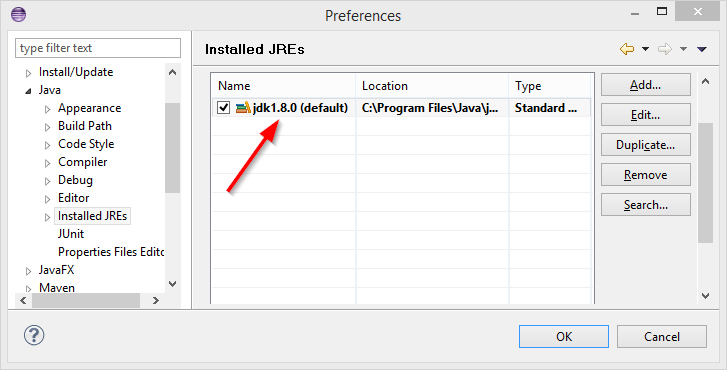
\includegraphics[height=7cm]{img/preferences-jdk}
	\end{figure}
	\item Navega a \textit{Java | Compiler}. Establece el \textbf{nivel de cumplimiento del compilador en 1.8} (Compiler compliance level).
	\begin{figure}[H]
		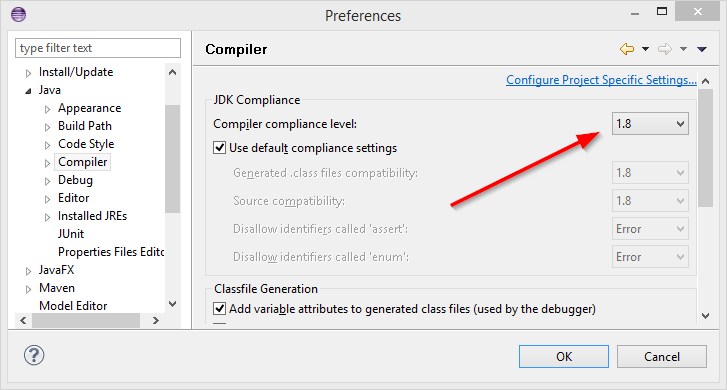
\includegraphics[height=7cm]{img/preferences-compliance}
	\end{figure}
	\item Navega hasta \textit{Java | JavaFX}. Especifica la ruta al ejecutable del Scene Builder.
	\begin{figure}[H]
		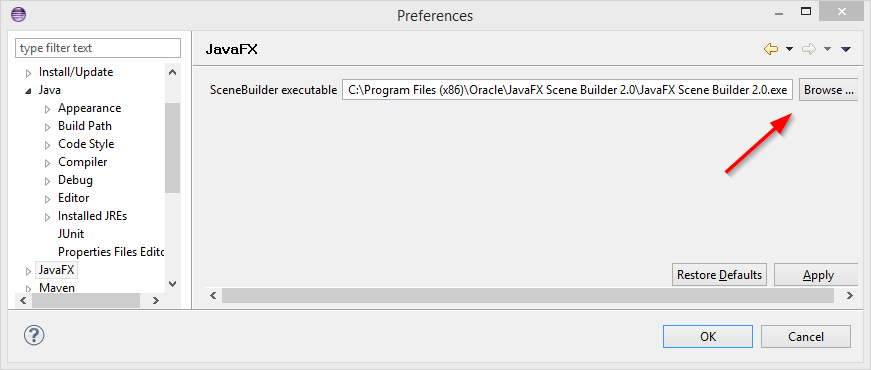
\includegraphics[height=7cm]{img/preferences-javafx}
	\end{figure}
	
\end{enumerate}


\section{Enlaces útiles}
Te podría interesar los siguientes enlaces:
\begin{enumerate}
	\item \textcolor{azul}{\href{https://docs.oracle.com/javase/8/docs/api/}{Java 8 API}} - Documentación (JavaDoc) de las clases estándar de Java
	\item \textcolor{azul}{\href{https://docs.oracle.com/javase/8/javafx/api/}{JavaFX 8 API}} - Documentación de las clases JavaFX
	\item  \textcolor{azul}{\href{https://controlsfx.bitbucket.io/}{ControlsFX API}} - Documentación (JavaDoc) - Documentación para el proyecto ControlsFX, el cual ofrece controles JavaFX adicionales
	\item \textcolor{azul}{\href{https://docs.oracle.com/javase/8/javafx/get-started-tutorial/get_start_apps.htm}{Oracle’s JavaFX}} Tutorials - Tutoriales oficiales de Oracle sobre JavaFX
\end{enumerate}
\texttt{¡Y ahora, manos a la obra!}

\section{Crea un nuevo proyecto JavaFX}
En Eclipse (con e(fx)clipse instalado) ve a \textit{File | New | Other…} y elige \textit{JavaFX Project}. Especifica el nombre del proyecto (ej. DireccionesApp) y aprieta \textit{Finish}.\\

	\begin{figure}[H]
		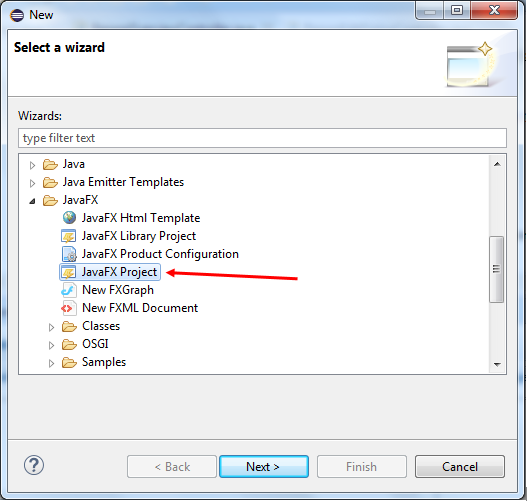
\includegraphics[width=8cm]{img/project1}
	\end{figure}
	\begin{figure}[H]
		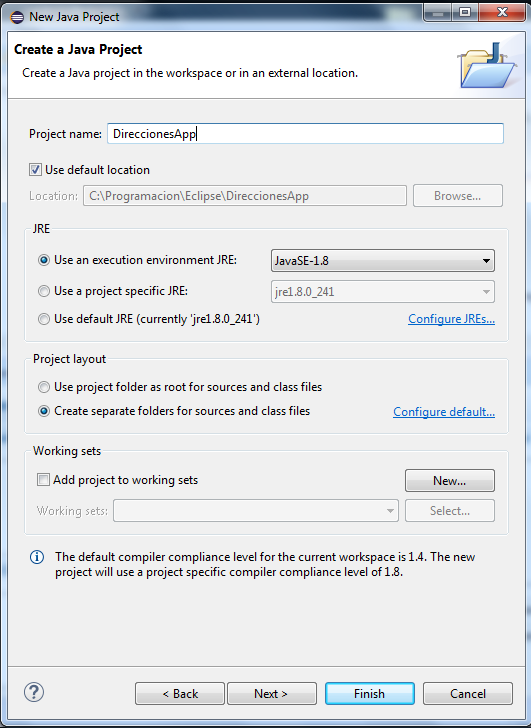
\includegraphics[width=8cm]{img/project2}
	\end{figure}

Borra el paquete \textit{application} y su contenido que ha sido creado automáticamente.

\subsection{Crea los paquetes}
Desde el principio vamos a seguir buenos principios de diseño de software. Algunos de estos principios se traducen en el uso de la arquitectura denominada \textcolor{azul}{\href{https://es.wikipedia.org/wiki/Modelo\%E2\%80\%93vista\%E2\%80\%93controlador}{Modelo-Vista-Controlador (MVC)}}. Esta arquitectura promueve la división de nuestro código en tres apartados claramente definidos, uno por cada elemento de la arquitectura. En Java esta separación se logra mediante la creación de tres paquetes separados.\\
En el ratón hacemos clic derecho en la carpeta \textit{src, New | Package:}
\begin{itemize}
	\item \textcolor{codigo}{\texttt{ch.makery.direcciones}} - contendrá la mayoría de clases de control (C).
	\item \textcolor{codigo}{\texttt{ch.makery.direcciones.model}} - contendrá las clases del modelo (M).
	\item \textcolor{codigo}{\texttt{ch.makery.direcciones.view}} - contendrá las vistas (V)
\end{itemize}
\textbf{Nota:} Nuestro paquete dedicado a las vistas contendrá también algunos controladores dedicados exclusivamente a una vista. Les llamaremos \textbf{controladores-vista}.

\section{Crea el archivo FXML de diseño}
Hay dos formas de crear la interfaz de usuario. Programándolo en Java o mediante un archivo XML. Si buscas en Internet encontrarás información relativa a ambos métodos. Aquí usaremos XML (archivo con la extensión .fxml) para casi todo. Encuentro más claro mantener el controlador y la vista separados entre sí. Además, podemos usar la herramienta de edición visual Scene Builder, la cual nos evita tener que trabajar directamente con el XML.\\
Haz clic derecho el paquete \textit{view} y crea un nuevo archivo FXML (\textit{New | Other | FXML | New FXML Document}) llamado \textcolor{codigo}{\texttt{PersonaOverview}}.
\begin{figure}[H]
	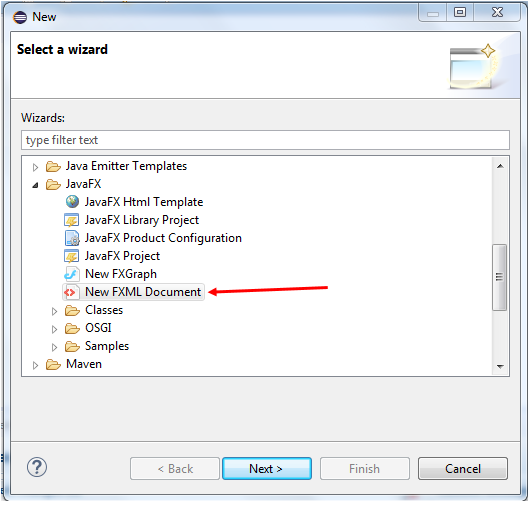
\includegraphics[width=8cm]{img/fxmlDocument}
\end{figure}
\begin{figure}[H]
	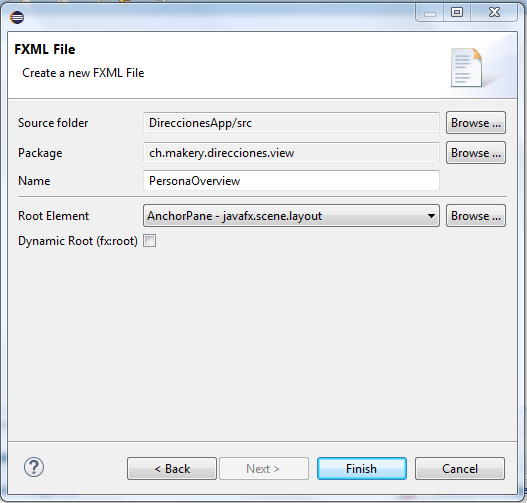
\includegraphics[width=8cm]{img/fxmlNombreDocument}
\end{figure}

\section{Diseño mediante Scene Builder}
\newtcolorbox{mybox}[1]{colback=red!5!white,
	colframe=red!75!black,fonttitle=\bfseries,
	title=#1}
\tcbset{colback=blue!5!white,colframe=blue!75!black}
\begin{tcolorbox}[leftrule=3mm]
	\textbf{Nota:} Si no puedes hacerlo funcionar, descarga las fuentes para esta parte del tutorial e inténtalo con el archivo fxml incluido.
\end{tcolorbox}

Haz clic derecho sobre PersonaOverview.fxml y elige \textit{Open with Scene Builder}. Ahora deberías ver el Scene Builder con un AnchorPane (visible en la jerarquía de componentes (herramienta Hierarchy) situada a la izquierda).
\begin{figure}[H]
	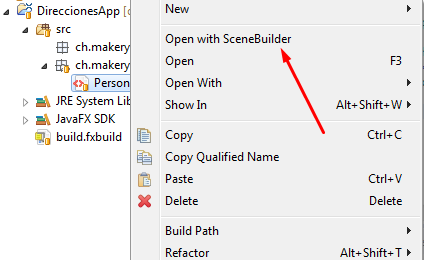
\includegraphics[width=7cm]{img/openSceneBuilder}
\end{figure}
Ya abierto Scene Builder
\begin{enumerate}
	\item Selecciona el \textit{AnchorPane} en tu jerarquía y ajusta el tamaño en el apartado Layout (a la derecha):
	\begin{figure}[H]
		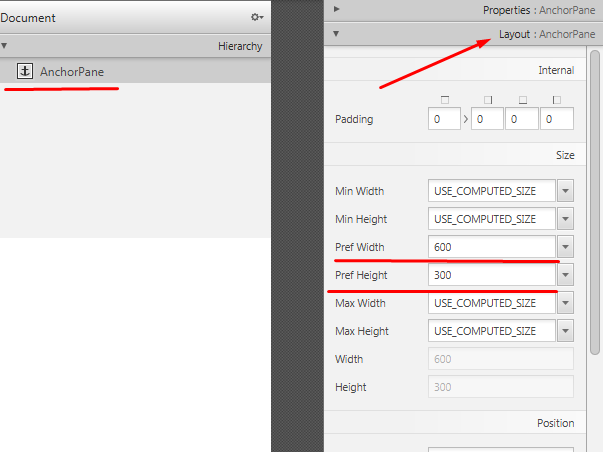
\includegraphics[width=11cm]{img/anchorPane}
	\end{figure}
	\item Añade un \textit{SplitPane (Horizontal Flow)} arrastrándolo desde la librería (Library) al área principal de edición. Haz clic derecho sobre el SplitPane en la jerarquía y elige Fit to Parent.
	\begin{figure}[H]
		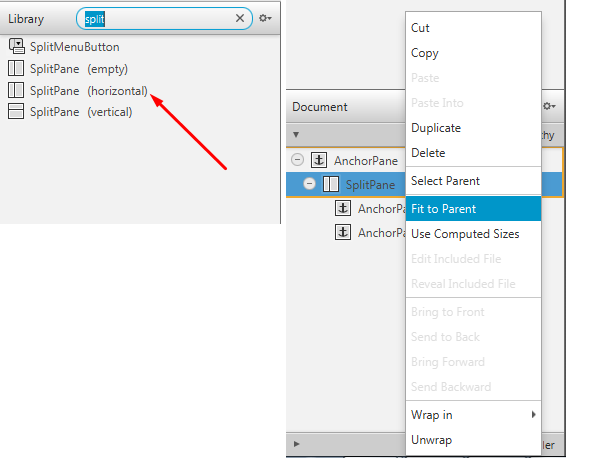
\includegraphics[width=11cm]{img/splitPane}
	\end{figure}

	\item Arrastra un TableView (bajo Controls) al lado izquierdo del SplitPane. Selecciona la TableView (no una sola columna) y establece las siguientes restricciones de apariencia (Layout) para la TableView. Dentro de un AnchorPane siempre se pueden establecer anclajes (anchors) para los cuatro bordes (\textcolor{azul}{\href{https://docs.oracle.com/javase/8/javafx/layout-tutorial/builtin_layouts.htm}{más información sobre Layouts}}).
		\begin{figure}[H]
		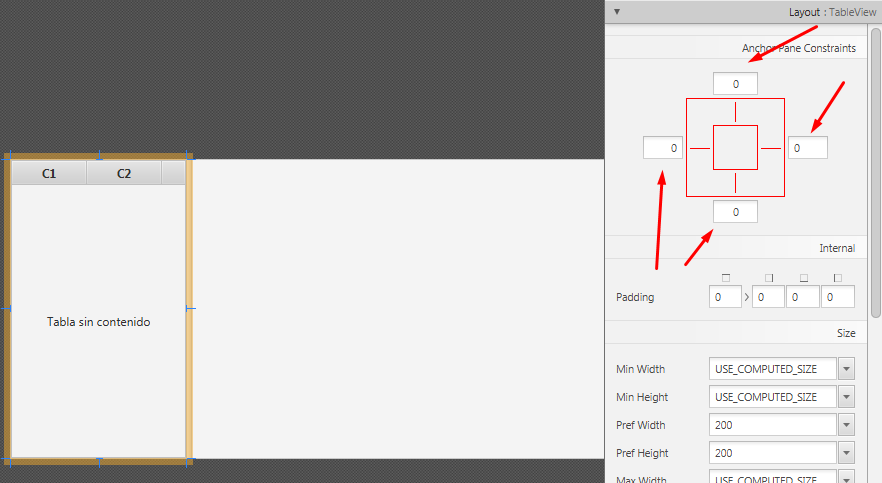
\includegraphics[width=14cm]{img/TableView}
	\end{figure}
	
	\item Ve al menú \textit{Preview | Show Preview in Window} para comprobar si se visualiza correctamente. Intenta cambiar el tamaño de la ventana. La TableView debería ajustar su tamaño al tamaño de la ventana, pues está “anclada” a sus bordes.
	
	\item Cambia el texto de las columnas (en \textit{Properties}) a “Nombre” y “Apellido”.
	\begin{figure}[H]
		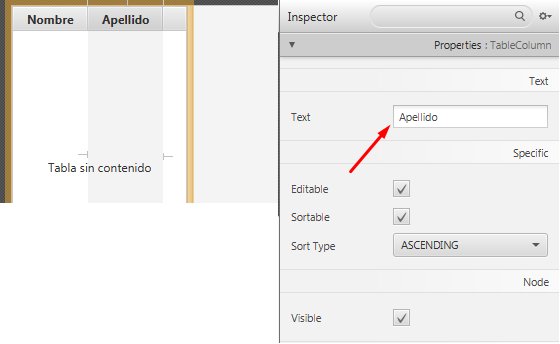
\includegraphics[width=10cm]{img/nombreApellido}
	\end{figure}
	\item Selecciona la \textit{TableView} y elige \textit{constrained-resize} para la \textit{Column Resize Policy} (en \textit{Properties}). Esto asegura que las columnas usarán siempre todo el espacio que tengan disponible.
	\begin{figure}[H]
		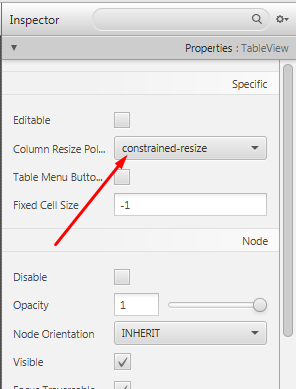
\includegraphics[width=7cm]{img/constraintRezise}
	\end{figure}
	\item Añade una \textit{Label} al lado derecho del \textit{SplitPane} con el texto “Detalles de Persona” (truco: usa la búsqueda en la librería para encontrar el componente \textit{Label}). Ajusta su apariencia usando anclajes.
	\begin{figure}[H]
		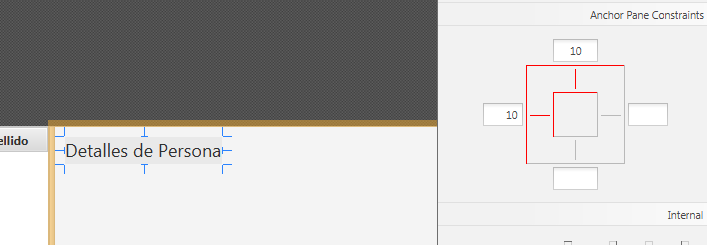
\includegraphics[width=13cm]{img/detallesPersona}
	\end{figure}
	\item Añade un \textit{GridPane} al lado derecho, selecciónalo y ajusta su apariencia usando anclajes (superior, derecho e izquierdo).
	\begin{figure}[H]
		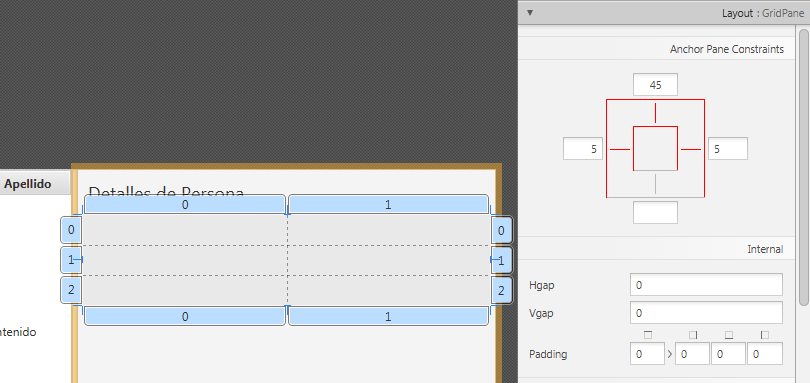
\includegraphics[width=16cm]{img/gridPane}
	\end{figure}
	\item Añade las siguientes etiquetas (\textit{Label}) a las celdas del GridPane.\\
	Nota: Para añadir una fila al \textit{GridPane} selecciona un número de fila existente (se volverá de color amarillo), haz clic derecho sobre el número de fila y elige “Add Row”.
	\begin{figure}[H]
		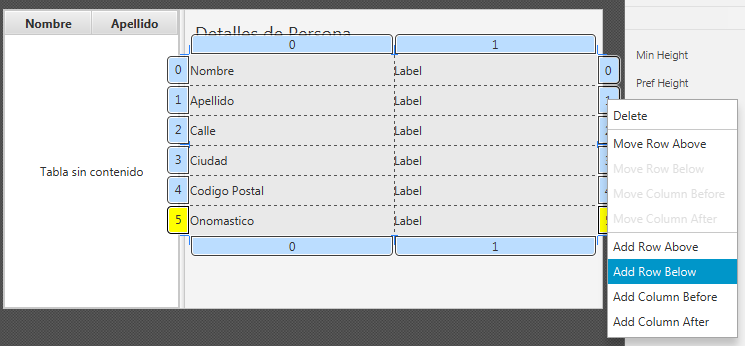
\includegraphics[width=14cm]{img/gridPaneAddRow}
	\end{figure}
	\item Añade tres botones a la parte inferior. Truco: Selecciónalos todos, haz click derecho e invoca \textit{Wrap In | HBox}. Esto los pondrá a los 3 juntos en un \textit{HBox}. Podrías necesitar establecer un espaciado spacing dentro del HBox. Después, establece también anclajes (derecho e inferior) para que se mantengan en el lugar correcto.
	\begin{figure}[H]
		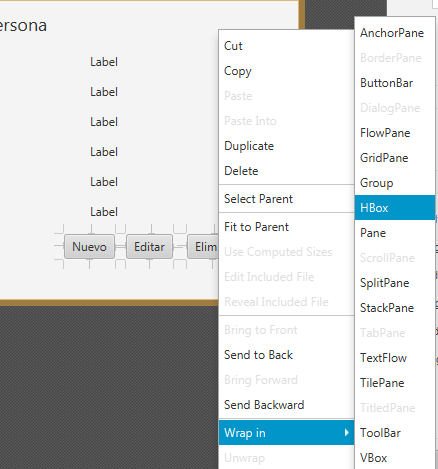
\includegraphics[width=10cm]{img/hBox}
	\end{figure}
	\begin{figure}[H]
		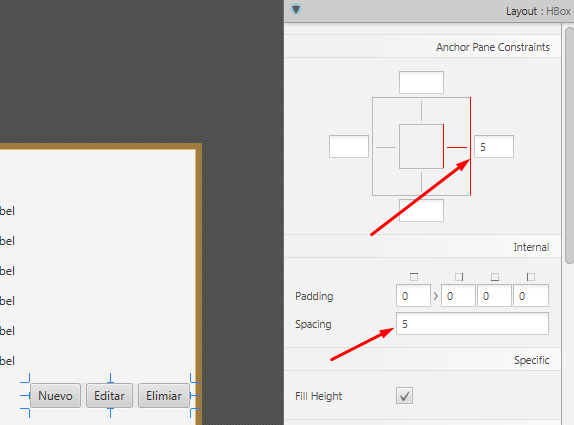
\includegraphics[width=10cm]{img/hBoxLayout}
	\end{figure}
	\item Ahora deberías ver algo parecido a lo siguiente. Usa el menú \textit{Preview} para comprobar su comportamiento al cambiar el tamaño de la ventana.
	\begin{figure}[H]
		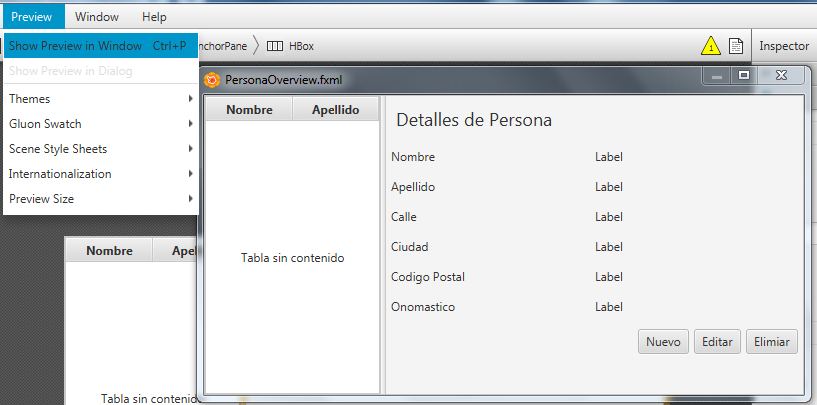
\includegraphics[width=14cm]{img/previewUno}
	\end{figure}


	\begin{tcolorbox}[leftrule=3mm]
		\textbf{Nota:} Guarda los cambios en SceneBuilder, el archivo se actualizará automáticamente en Eclipse, si esto no sucede, puedes presionar F5 para actualizar el archivo.
	\end{tcolorbox}

\end{enumerate}

\section{Crea la aplicación principal}
Necesitamos otro archivo FXML para nuestra vista raíz, la cual contendrá una barra de menús y encapsulará la vista recién creada \textcolor{codigo}{\texttt{PersonaOverview.fxml}}.
\begin{enumerate}
	\item Crea otro archivo FXML dentro del paquete view llamado \textcolor{codigo}{\texttt{RootLayout.fxml}}. Esta vez, elige BorderPane como elemento raíz.
	\begin{figure}[H]
		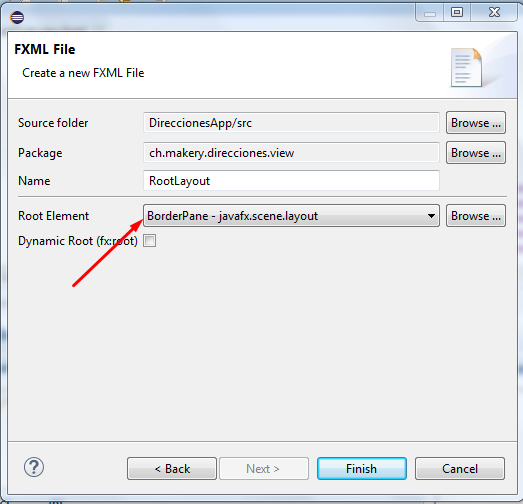
\includegraphics[width=11cm]{img/rootLayout}
	\end{figure}
	\item Abre \textcolor{codigo}{\texttt{RootLayout.fxml}} en el Scene Builder.
	\item Cambia el tamaño del \textit{BorderPane} con la propiedad \textit{\textit{Pref Width}} establecida en 600 y \textit{Pref Height} en 400.
	\begin{figure}[H]
		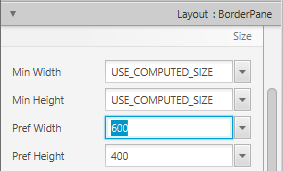
\includegraphics[width=9cm]{img/rootLayoutSize}
	\end{figure}
	\item Añade una \textit{MenuBar} en la ranura superior del \textit{\textit{BorderPane}}. De momento no vamos a implementar la funcionalidad del menú.
	\begin{figure}[H]
		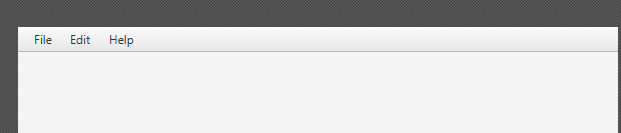
\includegraphics[width=9cm]{img/menuBarTop}
	\end{figure}
	
\end{enumerate}
\section{La clase principal en JavaFX}
Ahora necesitamos crear la clase java principal, la cual iniciará nuestra aplicación mediante \textcolor{codigo}{\texttt{RootLayout.fxml}} y añadirá la vista \textcolor{codigo}{\texttt{PersonOverview.fxml}} en el centro.

\begin{enumerate}
	\item Haz clic derecho en el proyecto y elige\textit{ New | Other | JavaFX | classes | JavaFX Main Class}.
	\begin{figure}[H]
		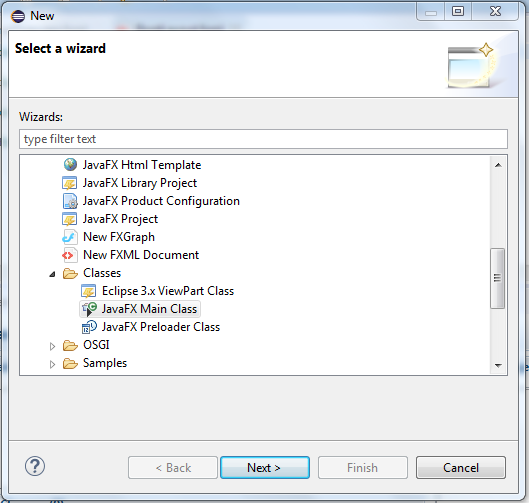
\includegraphics[width=11cm]{img/fxMainClass}
	\end{figure}
	
	\item Llama a esta clase \textcolor{codigo}{\texttt{MainApp}} y ponla en el paquete de controladores \textcolor{codigo}{\texttt{ch.makery.address}} (nota: este es el paquete padre de los paquetes \textcolor{codigo}{\texttt{view}} y \textcolor{codigo}{\texttt{model}}).
	\begin{figure}[H]
		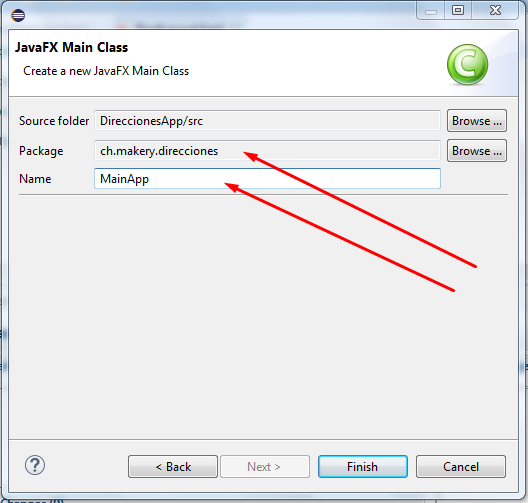
\includegraphics[width=11cm]{img/MainApp}
	\end{figure}
\end{enumerate}

La clase generada (\textcolor{codigo}{\texttt{MainApp.java}}) extiende a la clase \textcolor{codigo}{\texttt{Application}} y contiene dos métodos. Esta es la estructura básica que necesitamos para ejecutar una Aplicación JavaFX. La parte más importante para nosotros es el método \textcolor{codigo}{\texttt{start(Stage primaryStage)}}. Este método es invocado automáticamente cuando la aplicación es lanzada desde el método \textcolor{codigo}{\texttt{main}}.\\
Como puedes ver, el método \textcolor{codigo}{\texttt{start(...)}} tomo un \textcolor{codigo}{\texttt{Stage}} como parámetro. El gráfico siguiente muestra la estructura de cualquier aplicación JavaFX:
\begin{figure}[H]
	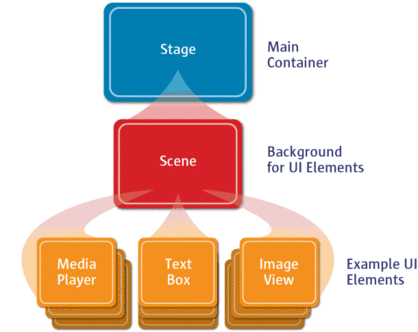
\includegraphics[width=8cm]{img/javafx-hierarchy}
	\caption*{Fuente de la imagen: \textcolor{azul}{\href{http://www.oracle.com}{http://www.oracle.com}}}
\end{figure}

Es como una obra de teatro: El \textcolor{codigo}{\texttt{Stage}} (escenario) es el contenedor principal, normalmente una ventana con borde y los típicos botones para maximizar, minimizar o cerrar la ventana. Dentro del \textcolor{codigo}{\texttt{Stage}} se puede añadir una \textcolor{codigo}{\texttt{Scene}} (escena), la cual puede cambiarse dinámicamente por otra \textcolor{codigo}{\texttt{Scene}}. Dentro de un \textcolor{codigo}{\texttt{Scene}} se añaden los nodos JavaFX, tales como \textcolor{codigo}{\texttt{AnchorPane}}, \textcolor{codigo}{\texttt{TextBox}}, etc.\\
Para tener más información puedes consultar \textcolor{azul}{\href{https://docs.oracle.com/javase/8/javafx/scene-graph-tutorial/scenegraph.htm}{Working with the JavaFX Scene Graph}}.\\
Abre el archivo \textcolor{codigo}{\texttt{MainApp.java}} y reemplaza todo su código con el código siguiente:


\begin{lstlisting}
// Hello.java
import javax.swing.JApplet;
import java.awt.Graphics;

public class Hello extends JApplet {
	public void paintComponent(Graphics g) {
		g.drawString("Hello, world!", 65, 95);
	}    
}
\end{lstlisting}
